\documentclass[12pt]{beamer}  
\usepackage{xeCJK}  
\usepackage{mathdots}  
\usepackage{graphicx}  
\usepackage{float}  
\usepackage{multirow}  
%\usepackage{cite}  
\usepackage{amsfonts, amsmath, mathrsfs, amsbsy, amssymb, dsfont,setspace}
\usepackage[square, comma, sort&compress, numbers]{natbib} 
%\usetheme{Warsaw}  
\usetheme{CambridgeUS}
\begin{document} 
\title{低秩特性和联合稀疏的减弱墙体回波方法研究}  
\author{黄臣}  
\date{\today}  
\frame{\titlepage}  
\begin{frame}
  \frametitle{Low-Rank}
  如果$\bf X$是一个$m$行$n$列的数值矩阵,$\rm {rank(}\bf X\rm {)}$是$\bf X$的秩,
  假如$\rm {rank(}\bf X\rm {)}$远小于$m$和$n$,则我们称$\bf X$是低秩矩阵。
  秩可以度量相关性,当用少数几个线性无关的向量就可以表示整个矩阵时,说明矩阵
  具有低秩特性,在图像上,低秩特性表现为图像上的基底(字典)数目会很少。具体
  应用可以为拿来去除照片中的噪点,电影中的雨丝也可以通过低秩表达的方式来去除。

  而在穿墙雷达成像中,来自前墙的回波也被认为是具有低秩特性的矩阵,因此可以
  使用相关方法进行去除墙体回波。
\end{frame}
\begin{frame}
  \frametitle{Low-Rank}
  低秩矩阵逼近(LRMA)的方法被应用在很多地方,\citep{Ren2016Image}采用了一种
  加权核范数最小化的方法,用于先验盲图像去模糊。\citep{Tang2016Radar}则提
  出了一种迭代软阈值算法,用于估计前墙回波的低秩矩阵和来自减少的测量集中
  的目标回波的稀疏矩阵。
\end{frame}
\begin{frame}
  \frametitle{SVD-based Approach}
\end{frame}
\begin{frame}[allowframebreaks]{References}
  \footnotesize
  %\scriptsize
  \bibliographystyle{ieeetr} 
  \bibliography{ct.bib} 
\end{frame}
\end{document}
\begin{frame}
  \frametitle{Compressive Sensing Based Scene Reconstruction}
\end{frame}
\begin{frame}
  \frametitle{Compressive Sensing Based Scene Reconstruction}
\end{frame}
\begin{frame}
  \frametitle{Compressive Sensing Based Scene Reconstruction}
\end{frame}
\begin{frame}
  \frametitle{Compressive Sensing Based Scene Reconstruction}
\end{frame}
\*begin{figure}[H]
  \centering
  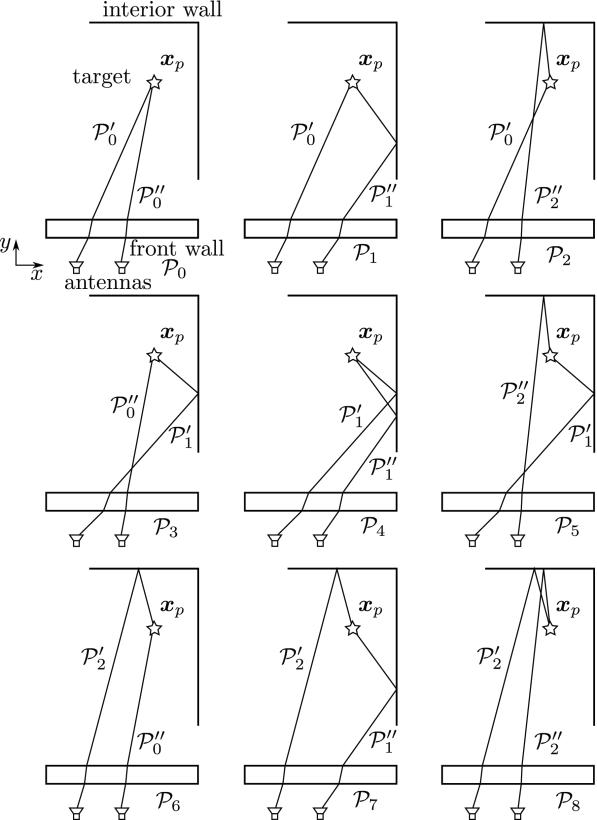
\includegraphics[width=0.5\textwidth]{fig2}
  \caption{CSI处理流程图}
\end{figure}
